\documentclass[twoside]{article}
\usepackage{algorithm}
\usepackage{algorithmic}
\usepackage{amssymb,amsmath,amsthm}
\usepackage{graphicx}
\usepackage{preamble}
\usepackage{natbib}
\usepackage{hyperref}
\usepackage{color}
\usepackage{wasysym}
\usepackage{subfigure}
\usepackage{tabularx}
\usepackage{booktabs}
\usepackage{bm}
\newcommand{\theHalgorithm}{\arabic{algorithm}}
\definecolor{mydarkblue}{rgb}{0,0.08,0.45}
\hypersetup{ %
    pdftitle={},
    pdfauthor={},
    pdfsubject={},
    pdfkeywords={},
    pdfborder=0 0 0,
    pdfpagemode=UseNone,
    colorlinks=true,
    linkcolor=mydarkblue,
    citecolor=mydarkblue,
    filecolor=mydarkblue,
    urlcolor=mydarkblue,
    pdfview=FitH}

\newcolumntype{x}[1]{>{\centering\arraybackslash\hspace{0pt}}m{#1}}
\newcommand{\tabbox}[1]{#1}


\setlength{\marginparwidth}{0.6in}
%%%%%%%%%%%%%%%%%%%%%%%%%%%%%%%%%%%%%%%%%%%%%%%%%%%%%%%%%%
%%%% EDITING HELPER FUNCTIONS  %%%%%%%%%%%%%%%%%%%%%%%%%%%
%%%%%%%%%%%%%%%%%%%%%%%%%%%%%%%%%%%%%%%%%%%%%%%%%%%%%%%%%%

%% NA: needs attention (rough writing whose correctness needs to be verified)
%% TBD: instructions for how to fix a gap ("Describe the propagation by ...")
%% PROBLEM: bug or missing crucial bit 

%% use \fXXX versions of these macros to put additional explanation into a footnote.  
%% The idea is that we don't want to interrupt the flow of the paper or make it 
%% impossible to read because there are a bunch of comments.

%% NA's (and TBDs, those less crucially) should be written so 
%% that they flow with the text.

\definecolor{WowColor}{rgb}{.75,0,.75}
\definecolor{SubtleColor}{rgb}{0,0,.50}

% inline
\newcommand{\NA}[1]{\textcolor{SubtleColor}{ {\tiny \bf ($\star$)} #1}}
\newcommand{\LATER}[1]{\textcolor{SubtleColor}{ {\tiny \bf ($\dagger$)} #1}}
\newcommand{\TBD}[1]{\textcolor{SubtleColor}{ {\tiny \bf (!)} #1}}
\newcommand{\PROBLEM}[1]{\textcolor{WowColor}{ {\bf (!!)} {\bf #1}}}

% as margin notes

\newcounter{margincounter}
\newcommand{\displaycounter}{{\arabic{margincounter}}}
\newcommand{\incdisplaycounter}{{\stepcounter{margincounter}\arabic{margincounter}}}

\newcommand{\fTBD}[1]{\textcolor{SubtleColor}{$\,^{(\incdisplaycounter)}$}\marginpar{\tiny\textcolor{SubtleColor}{ {\tiny $(\displaycounter)$} #1}}}

\newcommand{\fPROBLEM}[1]{\textcolor{WowColor}{$\,^{((\incdisplaycounter))}$}\marginpar{\tiny\textcolor{WowColor}{ {\bf $\mathbf{((\displaycounter))}$} {\bf #1}}}}

\newcommand{\fLATER}[1]{\textcolor{SubtleColor}{$\,^{(\incdisplaycounter\dagger)}$}\marginpar{\tiny\textcolor{SubtleColor}{ {\tiny $(\displaycounter\dagger)$} #1}}}


\usepackage{format/icml2013}
%\usepackage[left=1.00in,right=1.00in,bottom=0.25in,top=0.25in]{geometry} %In case we want larger margins for commenting purposes

%% For submission, make all render blank.
%\renewcommand{\LATER}[1]{}
%\renewcommand{\fLATER}[1]{}
%\renewcommand{\TBD}[1]{}
%\renewcommand{\fTBD}[1]{}
%\renewcommand{\PROBLEM}[1]{}
%\renewcommand{\fPROBLEM}[1]{}
%\renewcommand{\NA}[1]{#1}  %% Note, NA's pass through!
    
\begin{document}



\twocolumn[
\icmltitle{Bayesian Structure Discovery for Supervised Learning OR \\
Bayesian Structure Discovery for Regression\\
Kernel Structure Discovery OR \\
Discovering Structure in Kernels}
%\icmlauthor{Anonymous Authors}
%\icmladdress{ Unknown Institution}
%%%%FIXME - Make sure to update this!
\icmlkeywords{nonparametrics, gaussian process, machine learning, ICML, structure learning, extrapolation, regression, kernel learning, equation learning, supervised learning}
\vskip 0.3in
]

\begin{abstract}
%Gaussian process (GP) models are used widely and successfully.
%However, their effictiveness depends critically on choosing an appropriate family of kernels.
%This aspect of GP modeling has been sorely underdeveloped.
%In this paper, we introduce a procedure for automatically and efficiently searching through a large space of GP models.
The effectiveness of nonparametric regression models depends heavily on the choice of kernel.
We introduce a marginal-likelihood-based search over composite kernel structures which automatically constructs a structured Gaussian process model appropriate for the dataset.
We further demonstrate that such kernels often allow the posterior to be automatically decomposed into a sum of interpretable components, and in some cases allows long-range extrapolation.
We demonstrate this technique on several real datasets, and achieve state-of-the-art predictive performance.
\end{abstract}

\section{Introduction}

Supervised learning problems, such as classification and regression, learn a function ${\function : \InputSpace \to \OutputSpace}$ from some input (predictor) variables, $\InputVar$, to some output (response) variables, $\outputVar$.
Kernel based nonparametric models, such as support vector machines and Gaussian processes, have been one of the dominant paradigms for supervised machine learning over the last 20 years.
These methods depend on defining a kernel or covariance function, $\kernel : \InputSpace \times \InputSpace \to \Reals$ that specifies how similar or correlated outputs $\outputVar$ and $\outputVar'$ are at two inputs $\inputVar$ and $\inputVar'$, respectively.

A key challenge for kernel based methods is learning an appropriate kernel from data, and a great many papers have been written on this important topic\TBD{ cite kernel learning for SVMs and GP literature}.
In this paper we pose the problem of kernel learning as a problem in structure discovery from data.
Specifically, we focus on a Bayesian setting where the kernel specifies a covariance function for Gaussian process (GP) regression.

Traditionally, Gaussian process kernels have a few free hyperparameters which can be optimised (or inferred) from data.
However, it is well known that one can form composite kernels via combinations of simple base kernels (\eg squared exponential / radial basis function, periodic, linear etc.) and operations that preserve positive definiteness (\eg summation and multiplication).
We use this insight to define a simple grammar over composite kernels and we develop an automated search algorithm over the (exponentially large) space of kernels that can be derived from this grammar.
The search criterion is the marginal likelihood of the data for a given kernel, which is the driving term for Bayesian model comparison and selection in analogous structure discovery tasks such as graphical model learning\TBD{cite \eg Heckerman}.

Our experimental findings demonstrate that this structure discovery algorithm can automatically recover known kernel structure from data, and that on real data the learned structure of the kernel often corresponds to natural, interesting and interpretable decompositions of the unknown function.
Our hope is that the algorithm developed in this paper will help replace the current and often opaque art of kernel engineering with a more transparent science of automated kernel discovery\fTBD{maybe $\to$ conclusion}.

%Kernel-based nonparametric regression models have been widely and succesfully used over the last 20 years. [citations needed]
%As part of the development of this model class, a rich set of kernels have been developed for both continuous and structured data.
%Because different kernels reflect different properties of the function being modeled, the choice of kernel can have a large impact on the sorts of structure that can be expressed or discovered by the model.

%When approaching a new dataset, it is often not clear which kernel family is most appropriate, especially for non-experts.
%Often, a standard kernel family (typically squared-exponential) is chosen out of convenience, and kernel parameters are set by cross-validation or maximum marginal likelihood. [citations?]

%Sometimes the argument is made that since most kernels are universal (i.e. consistent in the limit), that the choice of kernel is not important[citation?].  However, our experiments demonstrate that for datasets of moderate size, predictive performance, extrapolation and interpretability all depend heavily on the choice of kernel. \TBD{RBG: Do people actually say the choice of kernel isn't important?  This sounds like a straw man...}

%\paragraph{Main contribution}
%In this paper, we introduce an automated search over composite kernels.
%We define the search space through a simple grammar consisting of a set of one-dimensional base kernels (squared-exp, periodic, linear, etc.) and operations which combine those kernels (add and multiply).
%Our objective function is the marginal likelihood of a Gaussian process model with the given kernel, conditioned on the data.

%We examine the composite kernels discovered by this search on several datasets, and demonstrate that they can recover known structure, and result in state-of-the-art predictive performance.  We further demonstrate that in some cases, the structured posterior can be automatically decomposed into a sum of interpretable components, e.g. in Figure \ref{fig:airline_decomp}. \TBD{RBG: Need to clarify that the contribution isn't that we can decompose it (that was in GPML), but that the decomposition is often interesting.}

%\section{Motivation}
%\TBD{RBG: Do we need a separate motivation section?  The introduction should motivate the work.}

%There is a large and mature literature on automatic structure discovery in unsupervised settings [citations including Josh].
%However, relatively little attention has been paid to automatic structure discovery in supervised learning.

%Similar searches over large model classes have been succesfully used in machine vision [cite Cox + Pinto].
%  This work respresents a step towards more data-based modeling, as opposed to proposing the model beforehand.
%In general, learning the model class from data seems superior proposing the model beforehand.
%In high dimensional problems, it is also hard for a practitioner to propose an appropriate model even after examining a dataset closely.
% Choosing a kernel family is also a stumbling block for non-experts who wish to use Gaussian Process models.

%Machine learning can be more data-driven, analogous to the high-thoughput approaches being used in biology. 

%\subsection{Convenience Priors}
%One of the main advantage of kernel methods, and Gaussian process regression in particular, is that the kernel can be used to specify interesting prior structure to the model.
%However, in practice, GPs are typically used with only the squared-exp kernel.
%[Apparently, this was one of Sholkopf's big dissapointment with GPs... is there a quote from him on this? -David]

%A frequent criticism of the Bayesian framework is that priors are often chosen purely for convenience. 
%Gaussian process priors may be a good examples of a model chosen for its tractability.
%However, specifying a compound kernel typically does not change the order of computational complexity of inference in Gaussian process models.
%The broad use of simple kernels may be simply due to the difficulty of determining which kinds of structure exist in the data.
%As well, even if one understands the structure present in a dataset, it is often non-obvious how to express that through a covariance function. 
%\TBD{RBG: Not sure we need this in the motivation. Is this basically just to answer the objection of why we don't consider the tradeoff between expressiveness and tractability?  Also, the prior can affect computational tractability if we're using approximate algorithms, so this makes it sound like we're only thinking about small datasets.}

%Automating the search over kernel structures should be especially useful in allowing pracitioners from a wide variety of backgrounds to use appropriate models for their data.
%Indeed, the authors were sometimes surprised by the kernels chosen by the automated search, and the elegant ways in which complex structure was expressed through simple combination of kernels.

\section{Expressing structure through kernels}
\label{sec:Structure}

Kernel functions $\kernel : \InputSpace \times \InputSpace \to \Reals$ can be used to define a measure of similarity between two points $\inputVar, \inputVar'$ in some space $\InputSpace$.
In the case of Gaussian process regression, the kernel defines a covariance function ${\KernelMatrix_{\inputVar \inputVar'} := \textrm{Cov}(\outputVar, \outputVar') = \kernel(\inputVar,\inputVar')}$.
%The kernel, $\kernel$, must define a valid covariance function\fTBD{expand me}; when this is the case $\kernel$ is said to be positive semi-definite (PSD).

Examples of commonly used kernels include squared exponential (SE), periodic (Per) and linear kernels (Lin) defined below\fTBD{If we add RQ then we have everything in one place}
\begin{eqnarray}
\kernel_\textrm{SE}(\inputVar, \inputVar') = & \sigma^2\exp\left(-\frac{(\inputVar - \inputVar')^2}{2\ell^2}\right) \\
\kernel_\textrm{PE}(\inputVar, \inputVar') = & \sigma^2\exp\left(-\frac{2\sin^2(\pi|\inputVar - \inputVar'|/p)}{\ell^2}\right) \\
\kernel_\textrm{LN}(\inputVar, \inputVar') = & \sigma_1^2 + \sigma_2^2(\inputVar - \ell)(\inputVar' - \ell).
\end{eqnarray}

When used within the context of GP regression, these kernels define priors on functions which place mass only on smooth, periodic or linear functions respectively.
\TBD{Reference a diagram - even if a composite kernel we can point out what the base kernel is doing.}

Valid kernels are closed under addition and multiplication with other valid kernels;
% \ie any algebraic composition of PSD kernels will define a PSD kernel.\fTBD{Cite theorem}
this allows one to create richly structured kernels from well understood base components.

\fTBD{Can probably kill simple kernel table. Focus on one table.}
%\newcommand{\fwb}{2.45cm}  % width
\newcommand{\fwh}{1.6cm}     % height
\begin{figure}[t]
\centering
\begin{tabular}{C{\fwb}C{\fwb}C{\fwb}}
%kernel & draws from GP & GP posterior \\
\rotatebox{90}{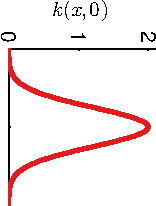
\includegraphics[width=\fwh,height=\fwb]{../figures/structure_examples/se_kernel}} &  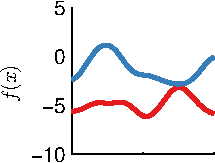
\includegraphics[width=\fwb,height=\fwh]{../figures/structure_examples/se_kernel_draws} & 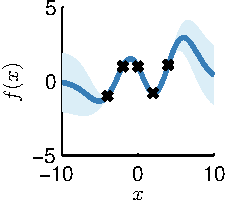
\includegraphics[width=\fwb,height=\fwh]{../figures/structure_examples/se_kernel_post} \\
squared-exp & \multicolumn{2}{c}{locally smooth} \\ \midrule
\rotatebox{90}{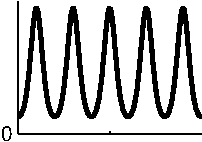
\includegraphics[width=\fwh,height=\fwb]{../figures/structure_examples/per_kernel}} &  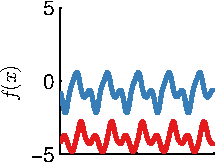
\includegraphics[width=\fwb,height=\fwh]{../figures/structure_examples/per_kernel_draws} & 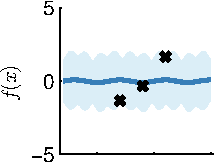
\includegraphics[width=\fwb,height=\fwh]{../figures/structure_examples/per_kernel_post} \\
periodic & \multicolumn{2}{c}{repeated structure} \\ \midrule
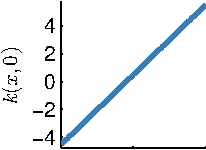
\includegraphics[width=\fwb,height=\fwh]{../figures/structure_examples/lin_kernel} &  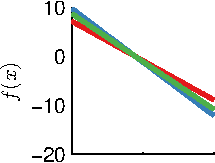
\includegraphics[width=\fwb,height=\fwh]{../figures/structure_examples/lin_kernel_draws} & 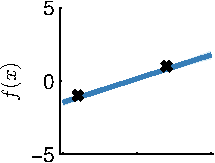
\includegraphics[width=\fwb,height=\fwh]{../figures/structure_examples/lin_kernel_post} \\
linear & \multicolumn{2}{c}{linear functions} \\ \midrule
\rotatebox{90}{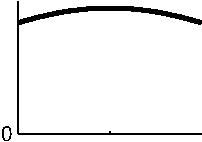
\includegraphics[width=\fwh,height=\fwb]{../figures/structure_examples/longse_kernel}} &  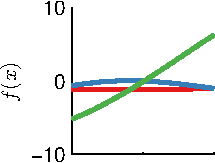
\includegraphics[width=\fwb,height=\fwh]{../figures/structure_examples/longse_kernel_draws} & 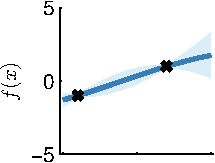
\includegraphics[width=\fwb,height=\fwh]{../figures/structure_examples/longse_kernel_post} \\
long-length SE & \multicolumn{2}{c}{slowly changing}
\end{tabular}
\caption{ Properties of basic kernels.  Left: base kernels. Centre:  draws from a \gp{} with that kernel.  Right: a GP posterior after conditioning on three datapoints.
\TBD{RBG: Do we need this figure?  It's pretty standard stuff, and it's largely subsumed by Figure 2.}}
\label{fig:basic_kernels}
\end{figure}

\newcommand{\fw}{2.6cm}
\begin{figure*}
\centering
\begin{tabular}{ccccc|c|c}
& & & & 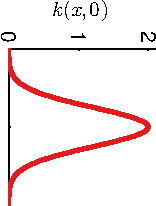
\includegraphics[width=\fw]{../figures/structure_examples/se_kernel} &  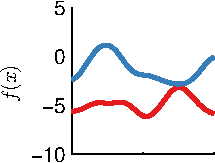
\includegraphics[width=\fw]{../figures/structure_examples/se_kernel_draws} & 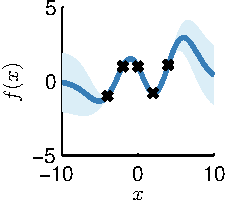
\includegraphics[width=\fw]{../figures/structure_examples/se_kernel_post} \\
& & & & 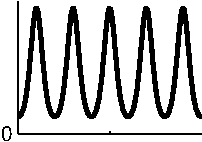
\includegraphics[width=\fw]{../figures/structure_examples/per_kernel} &  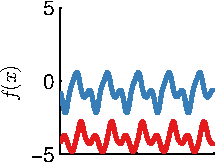
\includegraphics[width=\fw]{../figures/structure_examples/per_kernel_draws} & 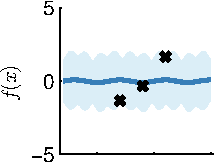
\includegraphics[width=\fw]{../figures/structure_examples/per_kernel_post} \\
& & & & 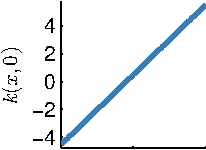
\includegraphics[width=\fw]{../figures/structure_examples/lin_kernel} &  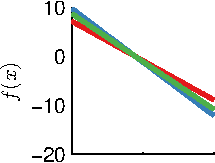
\includegraphics[width=\fw]{../figures/structure_examples/lin_kernel_draws} & 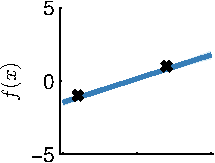
\includegraphics[width=\fw]{../figures/structure_examples/lin_kernel_post} \\
 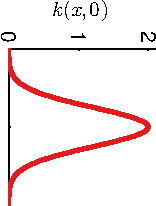
\includegraphics[width=\fw]{../figures/structure_examples/se_kernel} & $\times$ & 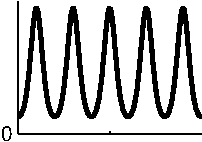
\includegraphics[width=\fw]{../figures/structure_examples/per_kernel} & = & 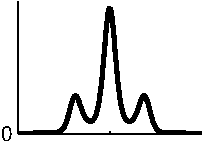
\includegraphics[width=\fw]{../figures/structure_examples/se_times_per} & 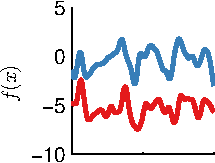
\includegraphics[width=\fw]{../figures/structure_examples/se_times_per_draws} & 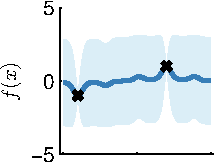
\includegraphics[width=\fw]{../figures/structure_examples/se_times_per_post} \\
  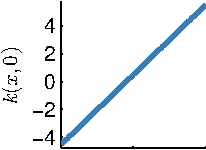
\includegraphics[width=\fw]{../figures/structure_examples/lin_kernel} & $\times$ & 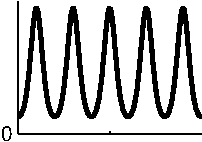
\includegraphics[width=\fw]{../figures/structure_examples/per_kernel} & = & 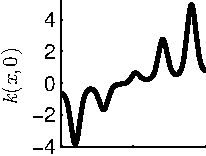
\includegraphics[width=\fw]{../figures/structure_examples/lin_times_per} & 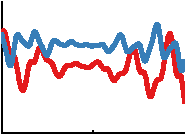
\includegraphics[width=\fw]{../figures/structure_examples/lin_times_per_draws} & 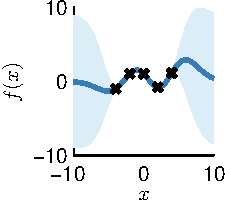
\includegraphics[width=\fw]{../figures/structure_examples/se_times_lin_post} \\
   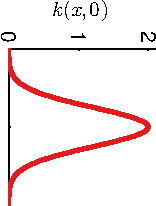
\includegraphics[width=\fw]{../figures/structure_examples/se_kernel} & $+$ & 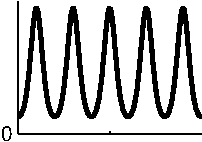
\includegraphics[width=\fw]{../figures/structure_examples/per_kernel} & = & 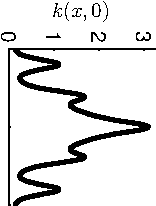
\includegraphics[width=\fw]{../figures/structure_examples/se_plus_per} & 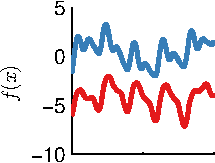
\includegraphics[width=\fw]{../figures/structure_examples/se_plus_per_draws} & 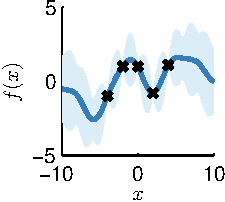
\includegraphics[width=\fw]{../figures/structure_examples/se_plus_per_post} \\
  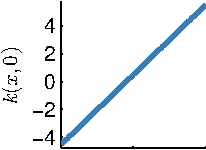
\includegraphics[width=\fw]{../figures/structure_examples/lin_kernel} & $+$ & 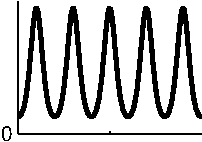
\includegraphics[width=\fw]{../figures/structure_examples/per_kernel} & = & 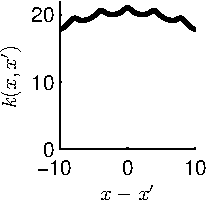
\includegraphics[width=\fw]{../figures/structure_examples/lin_plus_per} & 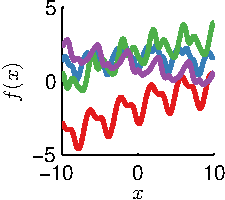
\includegraphics[width=\fw]{../figures/structure_examples/lin_plus_per_draws} & 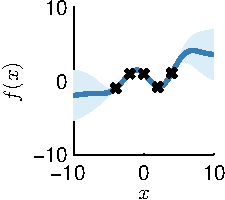
\includegraphics[width=\fw]{../figures/structure_examples/se_plus_lin_post} \\
   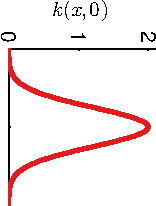
\includegraphics[width=\fw]{../figures/structure_examples/se_kernel} & $+$ & 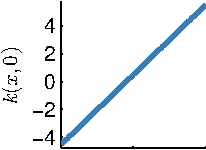
\includegraphics[width=\fw]{../figures/structure_examples/lin_kernel} & = & 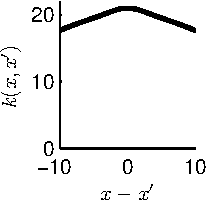
\includegraphics[width=\fw]{../figures/structure_examples/se_plus_lin} & 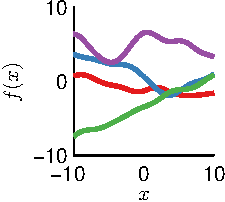
\includegraphics[width=\fw]{../figures/structure_examples/se_plus_lin_draws} & 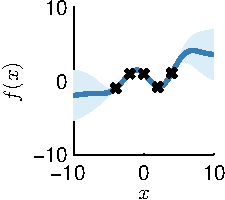
\includegraphics[width=\fw]{../figures/structure_examples/se_plus_lin_post} \\
   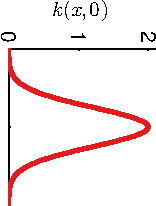
\includegraphics[width=\fw]{../figures/structure_examples/se_kernel} & $\times$ & 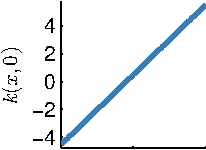
\includegraphics[width=\fw]{../figures/structure_examples/lin_kernel} & = & 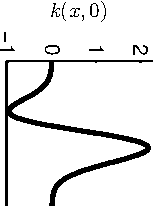
\includegraphics[width=\fw]{../figures/structure_examples/se_times_lin} & 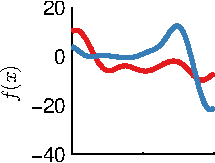
\includegraphics[width=\fw]{../figures/structure_examples/se_times_lin_draws} & \includegraphics[width=\fw]{../figures/structure_examples/se_times_lin_post} \\
base kernel & & base kernel & & combined kernel & draws from GP & GP posterior
\end{tabular}
\caption{ A draw from a sum of kernels corresponds to a sum of draws from the base kernels.  A draw from a product kernel prior has weaker long-range dependencies, and less long-range structure.
}
\label{fig:kernels}
\end{figure*}

\paragraph{Summation}

Summation of kernels corresponds to the summation of independent functions in the following sense.
Suppose ${\function_1 \dist \GP(0, \kernel_1)}$, and ${\function_2 \dist \GP(0, \kernel_2)}$ and are independent.
Then ${\function := \function_1 + \function_2 \dist \GP(0, \kernel_1 + \kernel_2)}$\footnotemark.
\footnotetext{Additionally, the posterior of the component functions conditioned on observations of the sum are analytically tractable. We make use of this in section\TBD{ add reference} and give derivations in the supplementary material.}

In one dimension, sums of kernels can express structure such as variational at multiple scales, or of summation of different function types.  Some examples can be found in Figure \ref{fig:kernels}.

In higher dimensions, summing kernels can correspond to decompositions of the form
\begin{equation}
\function((\inputVar_1, \inputVar_2)) = \function_1(\inputVar_1) + \function_2(\inputVar_2)
\end{equation}
\ie `independent' variation in different dimensions.
%
\begin{figure*}
\centering
\begin{tabular}{ccccc|c}
\hspace{-0.2cm}\includegraphics[width=0.2\textwidth]{../figures/additive_multi_d/additive_kernel_sum_p2.pdf} & \hspace{-0.4cm} + \hspace{-0.4cm} & 
\includegraphics[width=0.2\textwidth]{../figures/additive_multi_d/additive_kernel_sum_p1.pdf} & \hspace{-0.4cm} = \hspace{-0.4cm} & 
\includegraphics[width=0.2\textwidth]{../figures/additive_multi_d/additive_kernel.pdf} &
\includegraphics[width=0.2\textwidth]{../figures/additive_multi_d/sqexp_kernel.pdf} \\
$k_1(x_1, x_1')$ & & $k_2(x_2, x_2')$ & & $k_1(x_1,x_1') + k_2(x_2,x_2')$ &$k_1(x_1,x_1')k_2(x_2,x_2')$ \\
1D kernel & & 1D kernel & & sum of kernels & product of kernels \\ 
%& & & & & \\
%(Second Order) & & & & & Additive Kernel \\
$\downarrow$ & & $\downarrow$ & & $\downarrow$ & $\downarrow$ \\
\hspace{-0.2cm}\includegraphics[width=0.2\textwidth]{../figures/additive_multi_d/additive_kernel_draw_sum_p1.pdf}& \hspace{-0.4cm} + \hspace{-0.4cm}& 
\includegraphics[width=0.2\textwidth]{../figures/additive_multi_d/additive_kernel_draw_sum_p2.pdf}& \hspace{-0.4cm} = \hspace{-0.4cm}&
\includegraphics[width=0.2\textwidth]{../figures/additive_multi_d/additive_kernel_draw_sum.pdf} &
\includegraphics[width=0.2\textwidth]{../figures/additive_multi_d/sqexp_draw.pdf} \\
$f_1(x_1)$ & & $f_2(x_2)$ & & $f_1(x_1) + f_2(x_2)$ & $f(x_1, x_2)$ \\
draw from & & draw from & & draw from & draw from\\
1D GP prior & & 1D GP prior & & additive GP prior & product GP prior\\
%Draw from product kernel GP prior & Draw from additive kernel GP prior\\
\end{tabular}
\caption{A two-dimensional additive kernel, and a two-dimesnional product kernel.  Left: a draw from an additive kernel corresponds to a sum of draws from one-dimensional kernels.  Right: functions drawn from a product kernel prior have less long-range dependency.
%In this example, both kernels are composed of one dimensional squared-exponential kernels, but this need not be the case in general.
}
\label{fig:multi_d_additivity}
\end{figure*}

%
Figure \ref{fig:multi_d_additivity} demonstrates the decomposition across dimensions.

\paragraph{Interpretation}
Loosely speaking, a sum of kernels can be understood as an 'OR' operation: two points are considered similar if either kernel has a high value.
More precisely, we can interpret a sum of kernels as a concatenation of their features in the corresponding RKHS.

\paragraph{Multiplication}

Multiplication of kernels does not correspond to a simple composition of functions; here, we give some examples of the properties that arise from multiplication of kernels.

%but allows for the construction of different structures and is best understood on a case by case basis\fTBD{Better language?}.
%
%For example, multiplying base kernels of the same form that act upon different dimensions of $\InputSpace$ can create the multidimensional generalisations of these kernels; this is true of \eg SE and LN\TBD{ reference a picture}.
%
%Multiplying kernels of the same form in one dimension is often redundant \eg for SE kernels this just produces SE kernels with different parameters.
%\TBD{What is PE $\times$ PE?}
%However, multiplying kernels of different forms can give rise to interesting structures.

Multiplying a kernel $\kernel$ by the SE kernel allows the structures implied by $\kernel$ to vary smoothly according the lengthscale of the SE kernel.  This is shown in row 2 of Figure \ref{kernels}.
Multiplying a kernel by LN results in the amplitude of structures implied by $\kernel$ growing or shrinking linearly. This is shown in rows 4 and 5 of Figure \ref{kernels}.
%\fTBD{Could perhaps perversely claim that multiplying by periodic results in wiggles being added to previous structure?}
%
%\fTBD{Can we do more than just give examples}

%In general, multiplying kernels can be thought of as an `AND' operation when viewing kernels as a measure of similarity.
This arises since two points, $\inputVar,\inputVar'$, can only be considered similar by a product kernel function (\ie $\kernel_\textrm{prod}(\inputVar,\inputVar')$ is relatively large) if the points are considered similar by each component kernel function.

\paragraph{Interpretation}
Loosely speaking, multiplying kernels can be understood as an 'AND' operation: two points are considered similar only if both kernels have a high value.
More precisely, we can interpret a sum of kernels as a sum of the cartesian product of both kernels' features in the corresponding RKHS.

%\section{Gaussian Processes Priors}

%Gaussian processes are a flexible and tractable prior over functions, useful for solving regression and classification tasks\cite{rasmussen38gaussian}.
%The kind of structure which can be captured by a GP model is mainly determined by its \emph{kernel}: the covariance function.
%One of the main difficulties in specifying a Gaussian process model is in choosing a kernel which can represent the structure present in the data.
%For small to medium-sized datasets, the kernel has a large impact on modeling efficacy.
%\TBD{Note: The above paragraph is plagarized from my additive GP paper. -David} 

%
%The technique of constructing composite kernels using sums and products of existing kernels is not new \cite{rasmussen38gaussian} [more cites, Phil Hennig's astronomy work?].  
%However, the main contribution of this paper is to automate the search over kernel structures.

\section{Searching over structures}

\paragraph{A grammar for kernels}

The discussion above demonstrates that rich structure can be captured with summation and multiplication of simple base kernels.
We therefore consider searching over all kernel structures that can be expressed as sums and products of base kernels.

\begin{center}
\begin{tabular}{rccc}
\textrm{Replacement} & $\kernel_i$ & $\to$ & $\kernel'_i$\\% & $\forall\, \kernel' $\\
\textrm{Addition} & $\kernel_i$ & $\to$ & $\kernel_i + \kernel'_j$\\% & $\forall\, j,\kernel' $\\
\textrm{Multiplication} & $\kernel_i$ &  $\to$ & $\kernel_i \times \kernel'_j$\\% & $\forall\, j,\kernel'$\\
\end{tabular}
\end{center}

Details of the search algorithm are given in the supplementary material \TBD{For now}.

\paragraph{A greedy search algorithm}
In order to find the model with highest marginal likelihood, the base kernels and production rules generate a graph structure over kernel expressions and we follow a greedy search to traverse this graph.
This requires a method of scoring a kernel expression, which we achieve by using the Bayesian Information Criterion (BIC)\TBD{ cite me} as an estimate of the marginal likelihood of some data given the kernel expression\footnotemark.
\footnotetext{We also experimented with using a Laplace approximation to the marginal likelihood\TBD{ cite} but this was found to be less numerically stable and could not be computed if an optimiser failed to find a true optimum.}
Specifically, we optimise the marginal likelihood of the data given specific kernel parameters\TBD{ using LBFGS - cite?}, randomly restarting previously unoptimised kernel parameters.
This is then adjusted by the number of parameters optimised\footnotemark to compute the BIC\fTBD{formula?}.
\footnotetext{Adjustments were made for obvious parameter redundancy \eg multiplicative terms in products of kernels.}

The search then proceeds by scoring all base kernels applied to all input dimensions.
The highest scoring kernel is then expanded by applying all production rules, and these kernel expressions are scored.
The production rules are then applied to the highest scoring kernel expression and the search continues iteratively until some fixed depth.

\paragraph{Example expressions}

\TBD{Draw a picture to show what our model includes \ie polynomial regression, nonparametric `Fourier' decomposition, GAM, additive kernels.}

\section{Related Work}

\paragraph{Composite kernels in GP models} The technique of constructing composite kernels using sums and products of existing kernels is not new\fTBD{weak language}, and was demonstrated in detail in Chapter 5 of \cite{rasmussen38gaussian}, where the resulting posterior mean was also decomposed into a sum of component-wise means, although the posterior variance was not\fTBD{worth highlighting?}.

\cite{plate1999accuracy} constructs a GP with a composite kernel, adding a SE kernel along each dimension, and a SE-ARD kernel on all dimensions.  This model is motivated by the desire to specify the trade off between the interpretability of additive models and the flexibility of multiplicative models.

\paragraph{Compositional model search for unsupervised learning} \cite{grosse2012exploiting} performed a greedy search over a compositional model class for unsupervised learning.  Their models were composed of sums and element-wise products of random variables defined on matrices.  This model class contained a large number of existing unsupervised models as special cases.  Earlier work in unsupervised Bayseian structure discovery was done in \cite{kemp2008discovery}.

\paragraph{ANOVA Kernels}

Support vector regression with ANOVA decomposition kernels \cite{stitson1999support}

%\subsubsection{Smoothing spline ANOVA models}
A closely related procedure from the statistics literature is smoothing-splines ANOVA (SS-ANOVA)\cite{wahba1990spline, gu2002smoothing}.
An SS-ANOVA model is estimated as a weighted sum of splines along each dimension, plus a sum of splines over all pairs of dimensions, all triplets, etc, with each individual interaction term having a separate weighting parameter.
Because the number of terms to consider grows exponentially in the order, in practice, only terms of first and second order are usually considered.
Learning in SS-ANOVA is usually done via penalized-maximum likelihood with a fixed sparsity hyperparameter.
\TBD{We need to discuss how our model relates to this one - it's very similar!}

\paragraph{Hierarchical Kernel Learning}

%In "High-Dimensional Non-Linear Variable Selection through Hierarchical Kernel Learning", Bach
\cite{DBLP:journals/corr/abs-0909-0844} uses a regularized optimization framework to learn a weighted sum over an exponential number of kernels which can be computed in polynomial time.
The subsets of kernels considered by this method are restricted to be a \textit{hull} of kernels. In the setting we are considering in this paper, a hull can be defined as a subset of all terms such that if term $\prod_{j \in J} k_j(\bf x, x')$ is included in the subset, then so are all terms $\prod_{j \in J / i} k_j(\bf x, x')$, for all $i \in J$.
%For details, see \cite{DBLP:journals/corr/abs-0909-0844}.
%Given each dimension's kernel, and a pre-defined weighting over all terms, HKL performs model selection by searching over hulls of interaction terms.
% \subsubsection{All-subsets kernel with uniform weightings}
%In \cite{DBLP:journals/corr/abs-0909-0844}, Bach also fixes the relative weighting between orders of interaction with a single term $\alpha$, computing the sum over all orders by:
%\begin{equation}
%\label{eqn:uniform}
%k_{a}({\bf x, x'}) = v_D^2 \prod_{d=1}^D \left(1 + \alpha k_{d}(x_{d}, x_{d}') \right)
%\end{equation}
%which has computational complexity $O(D)$.
%However, this formulation forces the weight of all $n$th order terms to be weighted by $\alpha^n$.
%
The main difficulty with this approach is that hyperparameters are hard to set other than by cross-validation. 
%In contrast, our method optimizes the hyperparameters of each dimension's base kernel, as well as the relative weighting of each order of interaction. 



%A related functional ANOVA GP model\cite{kaufman2010bayesian} decomposes the \emph{mean} function into a weighted sum of GPs.
%However, the effect of a particular degree of interaction cannot be quantified by that approach.
%Also, computationally, the Gibbs sampling approach used in \cite{kaufman2010bayesian} is disadvantageous.

\paragraph{Genetic Searches over Kernel Structures}
A similar method was developed by \cite{diosan2007evolving} using SVMs in place of Gaussian processes, cross-validation error instead of marginal likelihood, and a genetic algorithm instead of a greedy search.  
In \cite{bing2010gp}, a genetic programming construction and optimization method was used to select a kernel for relevance vector machines.

\paragraph{Equation Learning}
A related body of work with similar goals are the various approaches to equation learning.  
For example, \cite{dzeroski1999equation} and \cite{washio1999discovering} attempt to learn parametric forms of equations to describe time series, or relations between quantities.  The advantage of a \gp{} approach is that 

\paragraph{Semiparametric Regression}
Semiparametric regression \TBD{add cites} attempts to combine interpretability with flexibility by building  a composite model out of an interpretable, parametric part (such as linear regression) and a ``catch-all'' nonparametric part (such as a \gp{} with an SE kernel).
Structure search has the same goal, but improves upon semiparametric regression in two ways.
First, construcing a compound model through structure in the kernel allows us to integrate over the parameters of the implicit components of the model.
Second, by automatically searching over components, we remove the limitation that the practictioner must be able to specify in advance the parametric form of any part of the model.


\paragraph{Multiple Kernel Learning}
There is a large body of work attempting to construct a rich kernel through a weighted sum of base kernels, including in \gp{} models.  
\cite{christoudias2009bayesian}
\TBD{cite more} 
However, these methods typically construct all kernels in advance, and simply reweight them.  This sort of approach would be inapplicable in our case, since our search space is exponential in our search depth, and we also must estimate the hyperparameters of each kernel.%One could imagine expanding our search for some fixed depth, instantiating a sum of all
%In the \gp{} framework,  showed how mixtures of kernels can be learnt by gradient descent in the Gaussian process framework.
%They call this \emph{Bayesian localized multiple kernel learning}.

\paragraph{Nonparametric kernel functions}

Since the complexity of our kernel is bounded only by the search depth, we could consider the structure search to be a non-parametric kernel model - in a sense, a doubly nonparametric model.  However, there has been some similar work along these lines in \cite{salakhutdinov2008using}, where a deep neural network was use to learn the kernel of a \gp{}.

%Hyperkernels \cite{ong2002hyperkernels}

\section{Decomposing a function}

Sums of kernels were shown in section~\ref{sec:Structure} to correspond to sums of independent function.
By splitting kernel expressions found by our search algorithm into additive components we can decompose a learned regression function.
This potentially allows us to separate causally independent processes that gave rise to data\TBD{ cite something / say nicely}.

Moreover, the posterior distribution over additive components is analytically tractable, allowing us to plot the individual components.
%\fTBD{If kept here, make notation consistent through paper}
The conditional distribution of a Gaussian $\function_1$ conditioned on its sum with another Gaussian $\vf = \vf_1 + \vf_2$ where $\vf_1 \sim \GP( \vmu_1, k_1)$ and $\vf_2 \sim \GP( \vmu_2, k_2)$ is given by
\begin{align}
\vf_1 | \vf \sim \mathcal{N} \big( & \vmu_1 + \vk_1^\star\tra (\vK_1 + \vK_2)\inv \left( \vf - \vmu_1 - \vmu_2 \right), \nonumber \\
& \vk_1 - \vk_1\tra (\vK_1 + \vK_2)\inv \vk_1 \big).
\end{align}
%and the covariance between the two components, conditioned on their sum is given by:
%\begin{align}
%\cov(\vf_1^\star, \vf_2^\star) | \vf = \vk_1^{\star\tra} (\vK_1 + \vK_2)\inv \vk_2^\star
%\end{align}
%Derivations can be found in the supplementary material.


We demonstrate the decompositions produced by our method on two time series.
We ran the search to a depth of 10 and use SE, PE, LN and RQ kernels\fTBD{make sure these are all defined}.

% %% --- Automatically generated by latex.py ---
% Exported at 2013-01-28 17:50:37.602844
\begin{table}[h!]
\begin{center}
\begin{tabular}{l | l l l}
   & \rotatebox{0}{ Description }  & \rotatebox{0}{ Parameters }  \\ \hline
SE & Squared-exponential  & lengthscale  \\
RQ & Rational Quadratic  & lengthscale, alpha  \\
LN & Linear  & none  \\
P & Piecewise Polynomial 1  & lengthscale  \\
MT & Mat\'{e}rn  & lengthscale  \\
\end{tabular}
\end{center}
\label{tbl:kernel_descriptions}
\end{table}


%The sorts of structure implied by complex kernel might not be immediately interpretable.
%However, there is one property of GPs that allows us to break down the signal into interpretable parts.
%Specifically, a function $f \sim \GP(0, k_1(x, x') + k_2(x,x')$, whose kernel is a sum of kernels, has the same distribution as a sum of two functions $\vf = \vf_1 + \vf_2$ where $\vf_1 \sim \GP( \vmu_1, k_1)$ and $\vf_2 \sim \GP( \vmu_2, k_2)$.
%In addition, the posterior distributions over individual components after conditioning on data are also analytically tractable.

\paragraph{Mauna Loa Atmospheric Carbon Dioxide}

We revisit a dataset explored in \cite{rasmussen38gaussian}, pages 120-126, where a kernel was hand-tailored to fit a GP model to the dataset.

Figures \ref{fig:mauna_grow} show the posterior of the increasingly appropriate model as the search depth increases on this dataset.
Note in particular that, while the data can be smoothly interpolated by simple kernels a single base kernel model, the extrapolations improve dramatically as the search depth increases.

Figure \ref{fig:mauna_decomp} shows the complete posterior of the maximum depth model together with the posteriors of the additive components.
The plot shows a very plausible extrapolation and highly interpretable components i.e.~a long-term trend, annual periodicity, medium-term deviations and short-term serially correlated `noise'.

\begin{figure}[h!]
\centering
\newcommand{\wmg}{2.66cm}  % width maunu growth
\newcommand{\hmg}{4cm}  % height maunu growth
\begin{tabular}{c}
 \includegraphics[width=\wmg,height=\hmg]{../figures/decomposition/03-mauna2003-s_max_level_0/03-mauna2003-s_all_small} 
 \includegraphics[width=\wmg,height=\hmg]{../figures/decomposition/03-mauna2003-s_max_level_1/03-mauna2003-s_all_small}
 \includegraphics[width=\wmg,height=\hmg]{../figures/decomposition/03-mauna2003-s_max_level_2/03-mauna2003-s_all_small}
\end{tabular}
\caption{Posterior mean and variance for different depths of kernel search.  In the first row, the function is only modeled as a locally smooth function, and the extrapolation is extemely poor.  In the second, a periodic component is added, and the extrapolation is better.  At depth 3, the kernel can capture most of the relevant structure, and is able to extrapolate reasonably. \TBD{RBG: (1) I think we somehow need to visualize the lengthscales, to make it obvious that the SE kernels really mean different things. (2) Why isn't SE + PE the correct answer?  In the second model, is the SE capturing part of the periodic component, forcing us to move to a locally periodic model?  (3) In general, in these figures, shouldn't we report the original form of the kernel rather than the expanded form?  It's not obvious how to get from 2 to 3 in one step.}}
\label{fig:mauna_grow}
\end{figure}

\begin{figure}[h!]
\newcommand{\wmgd}{9cm}  % width mauna growth decomp
\newcommand{\hmgd}{3cm}  % height mauna growth decomp
\begin{tabular}{c}
 \includegraphics[width=\wmgd,height=\hmgd]{../figures/decomposition/03-mauna2003-s_max_level_8/03-mauna2003-s_all} \\ = \\
 \includegraphics[width=\wmgd,height=\hmgd]{../figures/decomposition/03-mauna2003-s_max_level_8/03-mauna2003-s_2} \\ + \\
 \includegraphics[width=\wmgd,height=\hmgd]{../figures/decomposition/03-mauna2003-s_max_level_8/03-mauna2003-s_3} \\ + \\
% \includegraphics[width=\wmgd,height=\hmgd]{../figures/decomposition/03-mauna2003-s_max_level_8/03-mauna2003-s_4_zoom} \\ + \\
 \includegraphics[width=\wmgd,height=\hmgd]{../figures/decomposition/03-mauna2003-s_max_level_8/03-mauna2003-s_1} \\ + \\
 \includegraphics[width=8cm,height=\hmgd]{../figures/decomposition/03-mauna2003-s_max_level_8/03-mauna2003-s_resid}
\end{tabular}
\caption{First row: The posterior on the Mauna Loa dataset after a search of depth 8.  Subsequent rows: automatic decomposition of Mauna Loa data.  The signal has been automatically decomposed into long-term, yearly periodic, medium-term anomaly and short-term noise components, respectively.}
\end{figure}
\label{fig:mauna_decomp}

\paragraph{Airline passenger data}

\TBD{Give an intro to this dataset.}
Figures \ref{fig:airline_grow} and \ref{fig:airline_decomp} show the corresponding plots for the airline data set (\TBD{describe me!}).
\TBD{Make similar observations of good performance and perhaps draw attention to the selection of a linear kernel}.

\begin{figure}[h!]
\centering
\newcommand{\wag}{4cm}  % width airline growth
\newcommand{\hag}{4cm}  % height airline growth
\begin{tabular}{c}
 \includegraphics[width=\wag,height=\hag]{../figures/decomposition/01-airline-s_max_level_0/01-airline-s_all_small}
 \includegraphics[width=\wag,height=\hag]{../figures/decomposition/01-airline-s_max_level_1/01-airline-s_all_small} \\
 \includegraphics[width=\wag,height=\hag]{../figures/decomposition/01-airline-s_max_level_2/01-airline-s_all_small} 
 \includegraphics[width=\wag,height=\hag]{../figures/decomposition/01-airline-s_max_level_3/01-airline-s_all_small}
\end{tabular}
\caption{Posterior mean and variance for different levels of kernel search on the airline dataset.}
\label{fig:airline_grow}
\end{figure}


\begin{figure}[h!]
\centering
\newcommand{\wagd}{9cm}  % width airline growth decomp
\newcommand{\hagd}{4cm}  % height airline growth decomp
\begin{tabular}{c}
\includegraphics[width=\wagd,height=\hagd]{../figures/decomposition/01-airline-s_max_level_8/01-airline-s_all} \\ 
 = \\ 
 \includegraphics[width=\wagd,height=\hagd]{../figures/decomposition/01-airline-s_max_level_8/01-airline-s_1} \\
 + \\
 \includegraphics[width=\wagd,height=\hagd]{../figures/decomposition/01-airline-s_max_level_8/01-airline-s_2} \\
 + \\
 \includegraphics[width=\wagd,height=\hagd]{../figures/decomposition/01-airline-s_max_level_8/01-airline-s_3}
\end{tabular}
\caption{First row:  The airline dataset and posterior after a search of depth 8.  Rows 2-4: Additive decomposition of posterior into long-term smooth trend, yearly variation, and short-term noise.  Note that the variance of the noise grows over time, making this a heteroskedastic model.}
\label{fig:airline_decomp}
\end{figure}

%To evaluate the effectiveness of our method we performed two types of experiments.
%First, we examined the ability of our algorithm to discover useful structure in one-dimensional datasets.  Second, we examined the predictive performance of our model on multi-dimensional datasets.
% testing the ability of the algorithm to infer both an accurate regression function estimate and to produce an interpretable decomposition of a regression function.
%The accuracy experiments show that our method consistently matches or beats previous state of the art regression methods (\TBD{not yet statistically significantly within each experiment - more experiments currently running\ldots}).
%The decomposition experiments produce highly interpretable decompositions of time series data and highly plausible extrapolations; a particularly rare property of naively applied (linear) smoothers (\TBD{justify comment - e.g.~local linear is just linear, GP Sq-Exp nose dives towards the mean}).

\subsection{Multidimensional decomposition}

\begin{figure*}[h]
\centering
\begin{tabular}{ccc}
\includegraphics[width=0.3\textwidth]{../figures/additive_multi_d/interpretable_1st_order1.pdf} &
\includegraphics[width=0.3\textwidth]{../figures/additive_multi_d/interpretable_1st_order2.pdf}& 
\includegraphics[width=0.3\textwidth]{../figures/additive_multi_d/interpretable_2nd_order1.pdf}\\
\end{tabular}
\caption{One-dimensional decompositions of the concrete dataset posterior.  Left, Centre:  Green points indicate the original data, blue points are data after the mean contribution from the other dimensions' first-order terms has been subtracted.  The black line is the posterior mean of a GP with only one term in its kernel.  Right:  The posterior mean of a GP with only one second-order term in its kernel.}
\label{fig:interpretable functions}
\end{figure*}
%
Figure \ref{fig:interpretable functions} demonstrates that an additive posterior can be decomposed into a sum of functions across dimensions.


\section{Empirical evaluation}

In addition to producing highly interpretable decompositions of regression functions, our method also produces state of the art predictions in both extrapolation and interpolation tasks.

\subsection{Extrapolation}

\begin{figure}[h!]
\centering
\begin{tabular}{c}
\includegraphics[width=\columnwidth]{../figures/extrapolation_curves/01-airline-s-ex-curve.pdf}
\end{tabular}
\caption{Extrapolation performance.}
\end{figure}

Figure \ref{extrapolation} shows the learning curves of our method compared against simple linear regression and \gp{} regression with a SE kernel.  The amount of data in the 1D airline timeseries was increased by increments of 10\%. Both linear and SE regression plateau, while unbounded complexity of our method allows the model to continue to capture structure. 

\subsection{Interpolation}

To demonstrate the interpolation accuracy of our method we extend the comparison of \cite{duvenaud2011additive11} to include our method.
5 comparsion algorithms were evaluated on 5 datasets in terms of mean-squared (MSE) error and predictive likelihood using 10 fold cross validation.
Results are presented in tables \ref{tbl:Regression Mean Squared Error} and \ref{tbl:Regression Negative Log Likelihood}.
%
% --- Automatically generated by resultsToLatex2.m ---
% Exported at 28-Jan-2013 15:53:45
\begin{table*}[ht!]
\caption{{\small
Regression Mean Squared Error
}}
\label{tbl:Regression Mean Squared Error}
\begin{center}
\begin{tabular}{l | r r r r r}
Method & \rotatebox{0}{ bach  }  & \rotatebox{0}{ concrete  }  & \rotatebox{0}{ puma }  & \rotatebox{0}{ servo }  & \rotatebox{0}{ housing }  \\ \hline
Linear Regression & $1.031$ & $0.404$ & $0.641$ & $0.523$ & $0.289$ \\
GP GAM & $1.259$ & $0.149$ & $0.598$ & $0.281$ & $0.161$ \\
HKL & $\mathbf{0.199}$ & $0.147$ & $0.346$ & $0.199$ & $0.151$ \\
GP Squared-exp & $\mathbf{0.045}$ & $0.157$ & $0.317$ & $0.126$ & $\mathbf{0.092}$ \\
GP Additive & $\mathbf{0.045}$ & $\mathbf{0.089}$ & $\mathbf{0.316}$ & $\mathbf{0.110}$ & $0.102$ \\
%22-Jan & $\mathbf{0.513}$ & $\mathbf{0.089}$ & $\mathbf{0.312}$ & $\mathbf{0.095}$ & $\mathbf{0.091}$ \\
\hline
Structure Search & $\mathbf{0.044}$ & $\mathbf{0.087}$ & $\mathbf{0.315}$ & $\mathbf{0.102}$ & $\mathbf{0.082}$
\end{tabular}
\end{center}
\end{table*}
% End automatically generated LaTeX

% --- Automatically generated by resultsToLatex2.m ---
% Exported at 28-Jan-2013 15:53:45
\begin{table}[h!]
\caption{{\small
Regression Negative Log Likelihood
}}
\label{tbl:Regression Negative Log Likelihood}
\begin{center}
\begin{tabular}{l | r r r r r}
Method & \rotatebox{0}{ bach  }  & \rotatebox{0}{ concrete  }  & \rotatebox{0}{ puma }  & \rotatebox{0}{ servo }  & \rotatebox{0}{ housing }  \\ \hline
Linear Regression & $2.430$ & $1.403$ & $1.881$ & $1.678$ & $1.052$ \\
GP GAM & $1.708$ & $0.467$ & $1.195$ & $0.800$ & $0.457$ \\
GP Squared-exp & $\mathbf{-0.131}$ & $0.398$ & $0.843$ & $0.429$ & $0.207$ \\
GP Additive & $\mathbf{-0.131}$ & $\mathbf{0.114}$ & $\mathbf{0.841}$ & $\mathbf{0.309}$ & $0.194$ \\
22-Jan & $\mathbf{0.346}$ & $\mathbf{0.134}$ & $\mathbf{0.835}$ & $\mathbf{0.241}$ & $\mathbf{0.138}$ \\
28-Jan & $\mathbf{-0.141}$ & $\mathbf{0.065}$ & $\mathbf{0.840}$ & $\mathbf{0.265}$ & $\mathbf{0.059}$ \\
\end{tabular}
\end{center}
\end{table}
% End automatically generated LaTeX

%
Our method outperforms the other methods in all tests.

\TBD{Other versions of tests / learning curves}

\subsubsection{Data sets}


\paragraph{Bach Synthetic Dataset}
\fTBD{Too much text? Move to supplementary}
In addition to standard UCI repository datasets, we generated a synthetic dataset following the same recipe as \cite{DBLP:journals/corr/abs-0909-0844}.
% From a covariance matrix drawn from a Wishart distribution with 1024 degrees of freedom, we select 8 variables.
%We then construct the non-linear function $f(X) = \sum_{i=1}^4 \sum_{j=1+1}^4 X_i X_j + \epsilon$, which sums all 2-way products of the first 4 variables, and adds Gaussian noise $\epsilon$.
This dataset is one which can be predicted well by a kernel which is a sum of two-way interactions over the first 4 variables, ignoring the extra 4 noisy copies.
%
This dataset was designed by \cite{DBLP:journals/corr/abs-0909-0844} to demonstrate the advantages of HKL over a \gp{} with a SE-ARD kernel. 

%If the dataset is large enough, HKL can construct a hull around only those subsets of cross terms that are optimal for predicting the output.
%GP-ARD, in contrast, can only learn to ignore the noisy copy variables, but cannot learn to ignore the higher-term interactions between the predictive variables.
%However, a GP with an additive kernel can learn both to ignore irrelevant variables, and to ignore certain orders of interaction.
%In this example, the additive GP is able to recover the relevant structure.

[TODO: Describe concrete, pumadyn, servo and housing]

\subsection{Details of comparison methods}

\paragraph{Linear regression} was included as a baseline. A likelihood score was obtained by setting the noise variance to the empirical variance on the training set.

\paragraph{Generalized Additive Models} are models for which the posterior mean can be expressed $\expect[f(\vx)] = \sum_{d=1}^D f_d(x_d)$.  
In our experiments, this model is implemented through a GP whose kernel is a sum of sq-exp kernels across dimensions.  
This model, denoted GP GAM, was included to demonstrate that the gain in predictive performance was not simply due to the inclusion of additive structure.  \cite{hastie1990generalized}

\paragraph{Hierarchical Kernel Learning}	
HKL\footnote{Code for HKL available at \texttt{http://www.di.ens.fr/\textasciitilde fbach/hkl/}} was run using the all-subsets kernel, which corresponds to the same set of kernels as considered by the additive GP with a squared-exp base kernel.

\paragraph{Additive Gaussian Processes} \cite{duvenaud2011additive11} is a Gaussian process model whose kernel implicitly sums over all $2^D$ possible products of one-dimensional base kernels.  
However, this model's parameterization is not as flexible as the kernels expressible in our grammar.

\paragraph{Structure Search}
All of the experiments in this paper were performed using the standard GPML toolbox\footnote{Available at \texttt{http://www.gaussianprocess.org/gpml/code/}}; code to perform all experiments is available on github.

%$k = 1$, $D = 8$, kernels are SE and RQ (\TBD{currently running other experiments that may be more canonical}).
%We have extended the comparison of \cite{duvenaud2011additive11} to include our method.

%Some points for discussion
%\begin{itemize}
%\item Experiments just using SE kernel can outperform additive kernel surprisingly. This is presumably a regularisation effect of using a finite depth search and/or BIC. We could make this a more Bayesian result (i.e.~more a property of the model) by placing a prior on kernels that depends on the number of components.
%\item Need to discuss design choices e.g.~$k$, depth of search, base kernels.
%\end{itemize}

\section{Discussion}

Blessing of abstraction, doing lots with a small amount of data.

Extrapolation

\section{Conclusion}

In this paper, we introduced an automated search over composite kernels, defining the search space through a simple grammar consisting of a set of one-dimensional base kernels and operations which combine those kernels.

We examined the composite kernels discovered by this search on several datasets, and demonstrate that they can recover known structure, and result in state-of-the-art predictive performance.  We further demonstrated an automated decomposition of the posterior into a sum of interpretable components.

\NA{Machine learning can be more data-driven, analogous to the high-thoughput approaches being used in biology.}

%\section{Future Work}

%\TBD{RBG: Do we need this section?  Bill hates future work sections since they basically just give the reviewers a list of things to complain about.}

%\paragraph{Support Vector Machines} Structure search could be used to select kernels for support vector machines, using cross-validated prediction error as an objective function.

%However, it would be presumably quite difficult to learn the moderate number of kernel hyperparameters present in composite kernels using only cross-validation.

%\paragraph{Noise Models and Mean Functions}
%The models used in this paper all assumed Gaussian noise, as well a constant mean function for the Gaussian process.
%A more sophisticated approach might also define grammars over composite mean functions and noise models.
%However, in most cases, the covariance function can express structure that might be expressed in the mean function, and often in a more flexible way.
%The same can be said about noise models - for instance, a t-noise can be approximated by a sum of sq-exp kernels with very small lengthscales, but output variances which vary widely.


%\paragraph{Bayes model averaging}
%A natural extension of this work is to average over models in the grammar with a Bayes model averaging approach.
%This would mean augmenting our grammar with a prior over kernel structures, and approximately integrating over both structures and kernels.  

%In the first few levels of the search, where the difference between likelihoods of different kernel structures is usually high, model averaging might not make a substantial difference in terms of prediction.
%However, at deeper levels of the kernel search, integrating over structures and parameters would address overfitting concerns.

%\paragraph{Parsimony}
%Integrating over kernel structures raises the problem of reporting interpretable structures to the user.
%Currently, this is achieved through the use of the BIC complexity penalty, and reporting only the highest-scoring structure found.
%In experiments which used the more sophisticated Laplace approximation as a complexity penalty, the kernels found were more complicated.

%\paragraph{Bayesian Optimization} 
%The greedy search strategy used in this paper is rudimentary.  A natural extension of this work would be a model-based search over composite kernels, where the results of previous searches are used to propose informative directions.  This would be an example of ``meta-learning''.
%\cite{snoek2012practical} [also cite Lizotte, de Frietas]
%
%\paragraph{A Kernel between kernels}
%Placing a \gp{} model on the log-likelihood of different kernels would require constructing a kernel on kernels, as in \cite{ong2002hyperkernels}.

\subsubsection*{Acknowledgements}

\bibliographystyle{format/icml2013}
\bibliography{gpss}
\end{document}
